\documentclass[tikz,border=8pt]{standalone}
\usetikzlibrary{arrows.meta,positioning}

\input{grid_selection.texinc}

\definecolor{gridpoint}{RGB}{150,150,150}
\definecolor{neighborblue}{RGB}{32,105,180}

\begin{document}
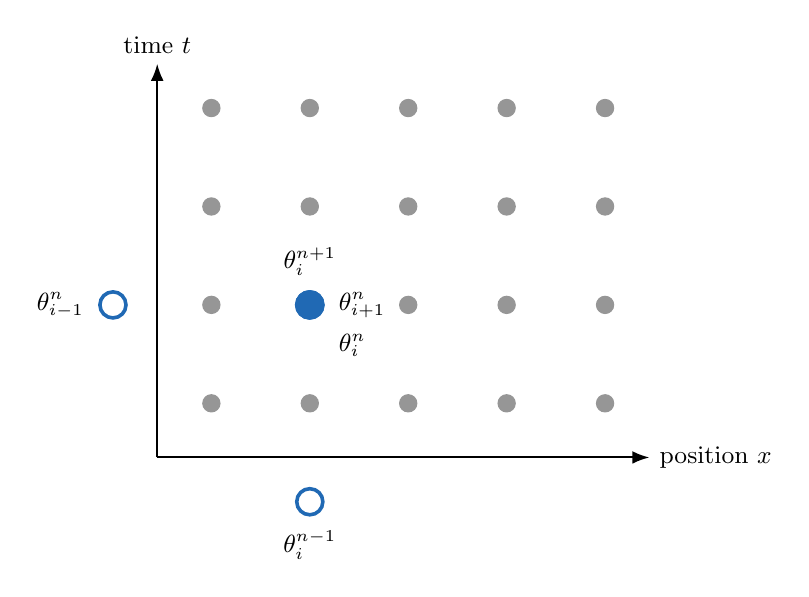
\begin{tikzpicture}[
    x=1.25cm,
    y=1.25cm,
    >=Latex,
    node/.style={circle,draw=gridpoint,fill=gridpoint,inner sep=2.2pt},
    neighbor/.style={circle,draw=neighborblue,line width=1.3pt,minimum size=8pt},
    center/.style={circle,draw=neighborblue,fill=neighborblue,minimum size=8pt},
    every node/.style={font=\small}
]
  \pgfmathtruncatemacro{\previousi}{\selectedi-1}
  \pgfmathtruncatemacro{\nexti}{\selectedi+1}
  \pgfmathtruncatemacro{\previousn}{\selectedn-1}
  \pgfmathtruncatemacro{\nextn}{\selectedn+1}

  \draw[->,line width=0.7pt] (-0.55,-0.55) -- (4.45,-0.55)
    node[right] {position $x$};
  \draw[->,line width=0.7pt] (-0.55,-0.55) -- (-0.55,3.45)
    node[above] {time $t$};

  \foreach \gridi in {0,...,4}
    \foreach \gridn in {0,...,3}
      \node[node] at (\gridi,\gridn) {};

  \node[neighbor] at (\previousi,\selectedn) {};
  \node[neighbor] at (\nexti,\selectedn) {};
  \node[neighbor] at (\selectedi,\previousn) {};
  \node[neighbor] at (\selectedi,\nextn) {};
  \node[center] at (\selectedi,\selectedn) {};

  \node[left=7pt] at (\previousi,\selectedn) {$\theta_{i-1}^n$};
  \node[right=7pt] at (\nexti,\selectedn) {$\theta_{i+1}^n$};
  \node[below=7pt] at (\selectedi,\previousn) {$\theta_i^{n-1}$};
  \node[above=7pt] at (\selectedi,\nextn) {$\theta_i^{n+1}$};
  \node[below right=7pt and 7pt] at (\selectedi,\selectedn) {$\theta_i^n$};
\end{tikzpicture}
\end{document}
